\documentclass[12pt]{article}

\usepackage[utf8]{inputenc}
\usepackage{graphicx}
\usepackage{fancyhdr}

\title{g55\_stack52 - 52 Slot 6-bit Stack}
\author{Group 55\\Juliette Regimbal (260657238)\\Qingzhou Yang (260687570)}
\date{March 20, 2017}
\pagenumbering{gobble}
\pagenumbering{arabic}
\pagestyle{fancy}

\begin{document}
\maketitle
\setlength{\parindent}{0ex}
\lhead{Group 55}
\rhead{Juliette Regimbal (260657238)\\Qingzhou Yang (260687570)}
\section{Circuit Description}
The \textit{g55\_stack52} circuit has 5 inputs and 4 outputs. There are two 6-bit inputs (\texttt{data} and \texttt{addr}), one 2-bit input (\texttt{mode}), and three 1-bit inputs (\texttt{enable, rst}, and \texttt{clk}). There are also two 6-bit outputs (\texttt{value} and \texttt{num}) and two 1-bit outputs (\texttt{empty} and \texttt{full}). 

\begin{figure}[h!t]
\centering
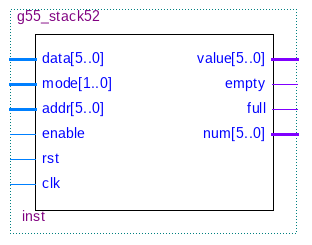
\includegraphics[scale=0.5]{graphics/stack_pinout.png}
\caption{\textit{g55\_stack52} Pinout}
\end{figure}

The stack has four modes of operation: NOP (no operation), INIT, POP, and PUSH. These occur synchronously with the clock signal \texttt{clk}, which typically is set to a 50MHz signal. The mode of operation is set with \texttt{mode}, with NOP, INIT, POP, and PUSH corresponding to 00, 01, 10, and 11 respectively. The selected operation will only occur when \texttt{enable} is high. Otherwise nothing will happen. \texttt{data} is an unsigned integer that serves as the data input for the POP operation. \texttt{addr} is an unsigned integer that selects the address of a certain slot in the stack. For example, an input of 000010 would correspond to slot 2. The value stored in the location specified by \texttt{addr} is available in \texttt{value}. \texttt{num} displays the number of entries in the stack up to a maximum of 52. \texttt{empty} and \texttt{full} are flags for when the stack has no entries and 52 entries respectively. \texttt{rst} is an asynchronous reset that sets all entries to 0 and empties the stack.\\

The NOP operation performs no operation. INIT uses all 52 possible slots in the stack, setting each to their index. For example, the zeroth entry has a value of 0, the first has a value of 1, and so on. POP clears the entry at the location specified by \texttt{addr} and shifts the entries with addresses greater than \texttt{addr} down by one. PUSH adds a value to the bottom of the stack (zeroth location) specified by the \texttt{data} input. All other entries are moved up one space. If the stack is full (52 entries), then the last is lost.\\

\section{Circuit Components}
As the \textit{g55\_stack52} circuit was done entirely in VHDL, there is no schematic diagram available. Each slot is its own component containing both a muxer (\textit{BUSMUX}) used to handle shifting entries up and down, and a flip flop (\textit{LPM\_FF}) that stores the value. Each slot (\textit{g55\_stack\_slot}) has a default value it initializes to. Within the \textit{g55\_stack52} circuit, a counter (\textit{LPM\_COUNTER}) is used to keep track of the number of slots used, a muxer (\textit{LPM\_MUX}) to route the value of the entry at \texttt{addr} to \texttt{value}. \textit{g55\_pop\_enable} is used to handle which slots will shift on POP and PUSH operations.\\

\section{Testing}

\section{Testbench and FPGA}
The testbench (\textit{g55\_lab3\_v2}) contains a \textit{g55\_stack52}, two \textit{g55\_7\_segment\_decoder} circuits, a \textit{g55\_mod13\_v2} circuit, and a \textit{g55\_debouncer} circuit. The enable is set to a pushbutton and goes through the debouncer before reaching the actual stack circuit. The \textit{g55\_mod13} takes \texttt{value} and sends the \texttt{Amod13} output to one of the \textit{g55\_7\_segment\_decoder} circuits and \texttt{floor13} to the other.\\

Altogether the testbench uses 989 logic elements as shown by the Flow Summary. With SignalTap II added to the circuit, the number of logic elements increases to 1569 logic elements. These values represent a use of 5\% and 8\% the total number of available logic elements respectively.

\end{document}